
\chapter{Arsitektur Container}
%\authors{Alfa Yohannis, Richwen Canady, Desfantio Wuidjaja, Vincenzo Matalino}

\section{Apa Itu Container?}

Container adalah paket perangkat lunak yang ringan, mandiri, dan dapat dieksekusi yang mencakup semua komponen yang diperlukan untuk menjalankan sebuah aplikasi, seperti kode, runtime, alat sistem, pustaka, dan konfigurasi. Berbeda dengan virtualisasi tradisional yang memerlukan sistem operasi terpisah untuk setiap mesin virtual, container berbagi kernel sistem operasi dari host. Pendekatan ini meningkatkan efisiensi, mengurangi overhead, dan mempercepat penerapan aplikasi.

Container menyediakan isolasi proses, memastikan bahwa setiap aplikasi berjalan secara independen meskipun berbagi sumber daya sistem yang sama. Isolasi ini meningkatkan keamanan serta menghilangkan konflik dependensi yang sering terjadi dalam model penerapan aplikasi tradisional. Dengan mengemas semua dependensi yang diperlukan, container menjamin konsistensi lingkungan dari tahap pengembangan hingga produksi.

Penggunaan container mendukung pengembangan aplikasi yang skalabel dan portabel. Karena semua dependensi aplikasi sudah termasuk dalam container, perangkat lunak dapat dijalankan secara konsisten di berbagai lingkungan, termasuk cloud, on-premise, dan infrastruktur hibrida. Hal ini meningkatkan keandalan serta mempercepat siklus pengembangan perangkat lunak.

Adopsi teknologi container telah merevolusi penerapan perangkat lunak modern dengan mendukung arsitektur microservices, di mana aplikasi dipecah menjadi layanan-layanan kecil yang independen. Pendekatan ini meningkatkan pemeliharaan dan skalabilitas, serta mengoptimalkan penggunaan sumber daya. Dibandingkan dengan mesin virtual, container menawarkan waktu startup yang lebih cepat dan konsumsi sumber daya yang lebih rendah, menjadikannya pilihan utama untuk aplikasi berbasis cloud dan pengembangan dengan pendekatan DevOps.

\section{Memahami Docker}

Docker adalah platform populer yang digunakan untuk mengembangkan, mendistribusikan, dan menjalankan aplikasi dengan teknologi containerisasi. Dengan Docker, aplikasi dapat dipisahkan dari infrastruktur, sehingga memungkinkan pengiriman perangkat lunak yang lebih cepat dan lebih andal.

Docker menyediakan kemampuan untuk mengemas dan menjalankan aplikasi dalam lingkungan yang terisolasi, yang disebut container. Setiap container mencakup semua dependensi yang diperlukan, seperti pustaka dan konfigurasi, sehingga memastikan aplikasi dapat berjalan secara konsisten di berbagai lingkungan tanpa konflik.

Dengan menggunakan Docker, proses deployment menjadi lebih efisien karena aplikasi dapat dipindahkan dari satu lingkungan ke lingkungan lain tanpa perubahan konfigurasi yang signifikan. Selain itu, Docker memungkinkan pengelolaan sumber daya yang lebih baik dan mendukung pengembangan berbasis microservices, di mana setiap layanan dapat dijalankan secara independen dalam container yang terpisah.




\section{Perbandingan Container dan Virtual Machine}

\begin{figure}[h]
	\centering
	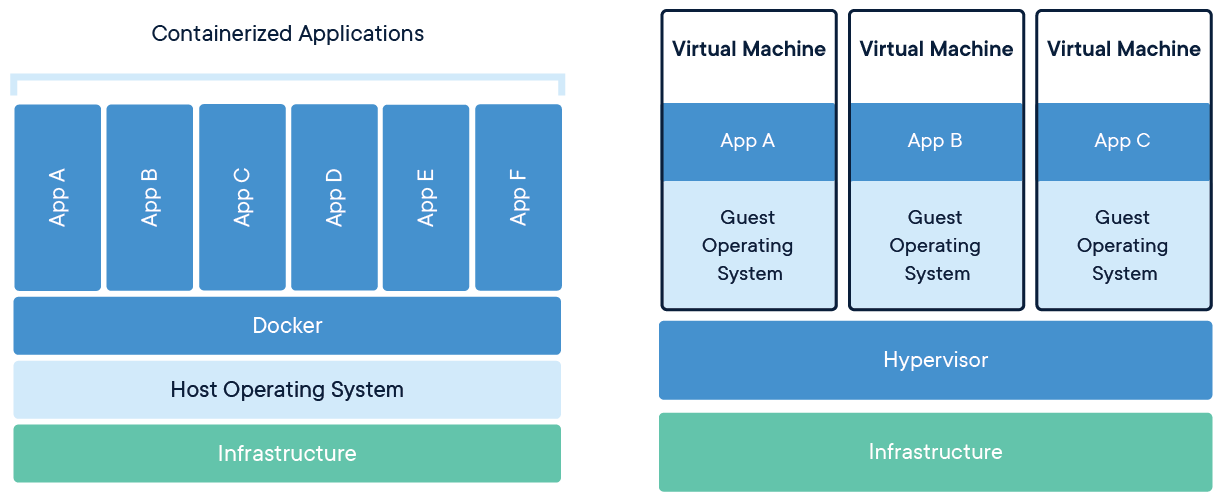
\includegraphics[width=\textwidth]{../images/container-vm.png}
	\caption{Perbedaan antara Container dan Virtual Machine}
	\label{fig:container-vm}
\end{figure}

Virtual machine (VM) dan container merupakan dua teknologi yang digunakan untuk menjalankan aplikasi dalam lingkungan yang terisolasi. Namun, keduanya memiliki pendekatan yang berbeda dalam hal arsitektur dan efisiensi sumber daya.

\subsection{Virtual Machine}
Virtual machine mencakup seluruh sistem operasi, termasuk kernel dan aplikasi, sehingga lebih berat dan membutuhkan lebih banyak sumber daya dibandingkan dengan container. Startup VM cenderung lebih lambat karena sistem operasi perlu dimuat sepenuhnya sebelum aplikasi dapat dijalankan.

VM bergantung pada teknologi \textbf{hypervisor}, yang mengelola beberapa virtual machine di satu mesin fisik dengan mengabstraksi sumber daya perangkat keras. Dengan adanya hypervisor, beberapa sistem operasi dapat berjalan secara independen di atas satu perangkat keras yang sama.

\subsection{Container}
Berbeda dengan VM, container berbagi kernel sistem operasi host, yang membuatnya lebih ringan dan membutuhkan lebih sedikit sumber daya. Karena tidak perlu memuat sistem operasi terpisah, container dapat dimulai lebih cepat dibandingkan dengan VM.

Keunggulan utama container adalah efisiensinya dalam menjalankan aplikasi berbasis microservices dan praktik DevOps. Dengan container, aplikasi dapat diisolasi secara independen tanpa overhead yang besar, memungkinkan pengelolaan dan skalabilitas yang lebih baik dalam lingkungan pengembangan dan produksi.


\section{Docker}

\begin{figure}[h]
	\centering
	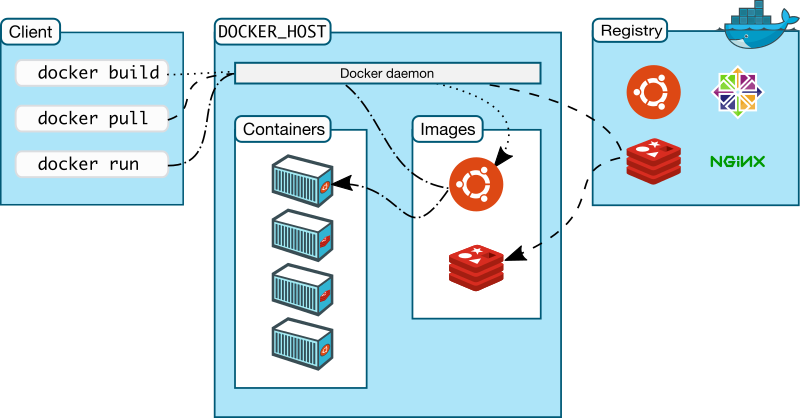
\includegraphics[width=\textwidth]{../images/docker.png}
	\caption{Struktur Docker}
	\label{fig:docker}
\end{figure}

Docker adalah platform yang memungkinkan pembuatan, pengiriman, dan menjalankan aplikasi dalam lingkungan container. Teknologi ini menyederhanakan proses deployment dengan mengisolasi aplikasi beserta dependensinya dalam unit yang ringan dan portabel.

\section{Komponen Docker}

Docker terdiri dari beberapa komponen utama yang bekerja bersama untuk mengelola container.

\subsection{Docker Engine}
Docker Engine adalah inti dari sistem Docker yang bertanggung jawab untuk menjalankan dan mengelola container. Komponen utama dalam Docker Engine meliputi:
\begin{itemize}
	\item \textbf{Docker Daemon}: Berjalan pada mesin host dan bertugas mengelola container, image, jaringan, serta volume penyimpanan.
	\item \textbf{Docker Client}: Antarmuka baris perintah (CLI) yang digunakan untuk berinteraksi dengan Docker Daemon.
\end{itemize}

\subsection{Images}
Image Docker adalah template baca-saja yang digunakan untuk membuat container. Image berisi semua yang dibutuhkan untuk menjalankan aplikasi, termasuk kode, dependensi, serta konfigurasi.

\subsection{Containers}
Container adalah instance yang dapat dijalankan dari image Docker. Container memungkinkan aplikasi berjalan dalam lingkungan yang terisolasi tanpa memerlukan sistem operasi terpisah, sehingga lebih ringan dibandingkan dengan virtual machine.

\subsection{Docker Registry}
Docker Registry adalah tempat penyimpanan image Docker. Salah satu contoh registry yang umum digunakan adalah \textbf{Docker Hub}, yang menyediakan berbagai image yang dapat diunduh dan digunakan sesuai kebutuhan.

Dengan menggunakan komponen-komponen ini, Docker menyediakan solusi yang efisien untuk pengelolaan dan distribusi aplikasi, memungkinkan pengembang untuk membangun lingkungan yang konsisten dari tahap pengembangan hingga produksi.

\section{Keunggulan Penggunaan Container}

Penggunaan container dalam pengelolaan aplikasi menawarkan berbagai keuntungan dibandingkan dengan metode tradisional seperti virtual machine. Beberapa keunggulan utama dari teknologi container adalah sebagai berikut:

\subsection{Portabilitas}
Container memastikan lingkungan aplikasi tetap konsisten di berbagai platform, baik itu di lingkungan pengembangan, pengujian, maupun produksi. Dengan demikian, aplikasi dapat dijalankan di berbagai sistem tanpa perlu konfigurasi ulang.

\subsection{Efisiensi}
Dibandingkan dengan virtual machine, container memiliki overhead yang lebih rendah karena tidak memerlukan sistem operasi terpisah untuk setiap instance. Dengan berbagi kernel sistem operasi host, penggunaan sumber daya menjadi lebih efisien.

\subsection{Skalabilitas}
Container memungkinkan aplikasi untuk dengan mudah disesuaikan berdasarkan permintaan. Dengan teknologi container orchestration seperti Kubernetes, container dapat diperbanyak atau dikurangi secara otomatis sesuai kebutuhan sistem.

\subsection{Isolasi}
Setiap container berjalan dalam lingkungan yang terisolasi, sehingga mencegah konflik antar aplikasi yang berjalan dalam satu sistem. Isolasi ini juga meningkatkan keamanan karena container tidak saling mempengaruhi satu sama lain.

\subsection{CI/CD (Continuous Integration/Continuous Deployment)}
Container mendukung otomatisasi dalam pengembangan perangkat lunak dengan mempermudah proses integrasi, pengujian, dan deployment. Dengan container, pengembang dapat membangun pipeline CI/CD yang lebih cepat dan andal, memungkinkan iterasi perangkat lunak yang lebih efisien.

Dengan keunggulan-keunggulan ini, teknologi container menjadi pilihan utama dalam pengembangan perangkat lunak modern, terutama dalam lingkungan berbasis cloud dan arsitektur microservices.



\section{Kekurangan Penggunaan Container}

Meskipun container menawarkan berbagai keunggulan, terdapat beberapa tantangan yang perlu diperhatikan dalam penggunaannya. Berikut adalah beberapa kekurangan utama dari teknologi container:

\subsection{Keamanan}
Container berbagi kernel sistem operasi host, yang dapat menimbulkan risiko keamanan jika tidak dikonfigurasi dengan benar. Kerentanan dalam satu container berpotensi memengaruhi seluruh sistem, terutama jika isolasi antar container tidak diterapkan dengan baik.

\subsection{Persistensi}
Pengelolaan aplikasi berbasis stateful dalam lingkungan container dapat menjadi tantangan. Karena container bersifat ephemeral (tidak permanen), data yang disimpan di dalamnya dapat hilang saat container dihentikan atau dihapus. Oleh karena itu, diperlukan solusi penyimpanan eksternal seperti volume atau database yang mendukung persistensi data.

\subsection{Jaringan}
Konfigurasi jaringan dalam lingkungan container bisa menjadi kompleks, terutama dalam skenario yang melibatkan banyak container yang harus berkomunikasi satu sama lain. Manajemen jaringan dalam skala besar memerlukan pendekatan yang matang, termasuk penggunaan alat orkestrasi seperti Kubernetes untuk mengelola komunikasi antar container.

\subsection{Kompatibilitas}
Tidak semua aplikasi cocok untuk dijalankan dalam container. Aplikasi yang bergantung langsung pada perangkat keras atau memiliki arsitektur yang sangat monolitik mungkin memerlukan adaptasi tambahan sebelum dapat di-containerisasi dengan baik.

Meskipun memiliki beberapa keterbatasan, teknologi container tetap menjadi pilihan utama dalam banyak skenario pengembangan perangkat lunak. Dengan konfigurasi yang tepat dan strategi mitigasi risiko, kelemahan-kelemahan tersebut dapat diminimalkan untuk memaksimalkan manfaat container dalam pengelolaan aplikasi modern.


\section{Contoh Penerapan Container}

Teknologi container digunakan dalam berbagai skenario untuk meningkatkan efisiensi, skalabilitas, dan konsistensi dalam pengembangan serta pengelolaan aplikasi. Berikut adalah beberapa contoh penerapannya:

\subsection{Aplikasi Web}
Container memungkinkan deployment layanan web dalam lingkungan yang konsisten di berbagai platform. Dengan container, konfigurasi server dan dependensi dapat dikemas dalam satu unit yang mudah didistribusikan dan dijalankan di lingkungan pengembangan, pengujian, maupun produksi.

\subsection{Arsitektur Microservices}
Container sangat mendukung penerapan arsitektur microservices, di mana setiap layanan berjalan secara independen dalam container yang terisolasi. Dengan pendekatan ini, pengelolaan, pemeliharaan, dan penskalaan layanan menjadi lebih fleksibel dan efisien.

\subsection{Lingkungan Pengembangan}
Penggunaan container dalam lingkungan pengembangan memastikan bahwa setiap anggota tim bekerja dalam lingkungan yang seragam. Dengan container, masalah terkait perbedaan sistem operasi atau konfigurasi dapat dihindari, sehingga pengembangan dan pengujian dapat berjalan lebih lancar.

\subsection{Pemrosesan Data}
Container digunakan untuk menjalankan tugas pemrosesan data dalam lingkungan yang terisolasi. Teknologi ini memungkinkan eksekusi pipeline data secara efisien tanpa perlu khawatir tentang konflik dependensi atau perbedaan konfigurasi sistem.

\subsection{Pipeline CI/CD}
Container mendukung otomatisasi dalam siklus pengembangan perangkat lunak dengan memungkinkan penerapan pipeline CI/CD (Continuous Integration/Continuous Deployment). Dengan container, proses build, pengujian, dan deployment dapat dilakukan secara lebih cepat dan konsisten di berbagai lingkungan.

Dengan berbagai penerapan ini, container menjadi solusi utama dalam pengembangan perangkat lunak modern, memungkinkan aplikasi yang lebih modular, fleksibel, dan dapat dijalankan di berbagai infrastruktur tanpa hambatan yang signifikan.


\section{Kesimpulan}

Penggunaan container, terutama dengan Docker, telah merevolusi cara pengembangan dan deployment perangkat lunak. Teknologi ini menyediakan lingkungan yang ringan, konsisten, dan terisolasi, memungkinkan aplikasi dijalankan dengan efisien di berbagai platform tanpa bergantung pada konfigurasi spesifik sistem.

Meskipun terdapat beberapa tantangan dalam penerapan container, keunggulannya sering kali lebih dominan, terutama dalam arsitektur berbasis microservices dan sistem yang memerlukan skalabilitas tinggi. Container memungkinkan pengelolaan aplikasi yang lebih fleksibel, mempercepat siklus pengembangan, serta meningkatkan efisiensi dalam distribusi dan deployment perangkat lunak.

Dengan semakin luasnya adopsi teknologi container, ekosistem pengembangan perangkat lunak terus berkembang menuju solusi yang lebih modular, portabel, dan mudah dikelola, menjadikannya pilihan utama dalam pengelolaan aplikasi modern.



\section{Contoh Aplikasi Container}

Untuk mendemonstrasikan penggunaan container, berikut adalah contoh sistem yang terdiri dari beberapa \textit{container Docker} yang berjalan secara independen dan berkomunikasi melalui jaringan \texttt{bridge}. Setiap layanan memiliki peran spesifik dalam pengelolaan data karyawan dan performanya, serta menyediakan antarmuka untuk administrasi database. Kode program dapat ditemukan di \url{https://github.com/alfa-yohannis/software-architecture/tree/main/code/chapter02/java-example}.

\begin{figure}[h]
	\centering
	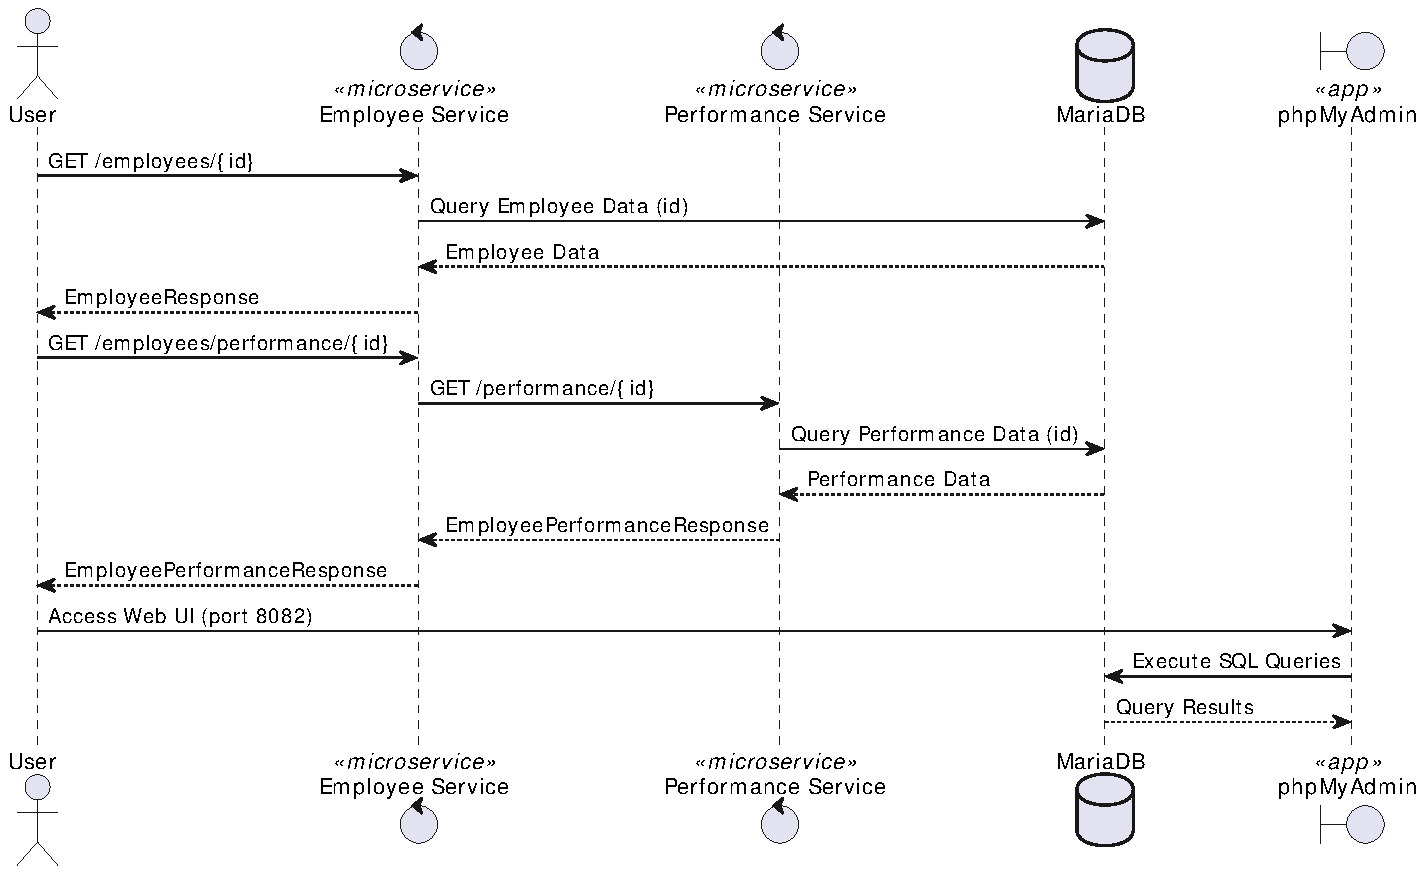
\includegraphics[width=\textwidth]{../images/out/microservices-employees}
	\caption{Struktur Docker}
	\label{fig:employee_performance}
\end{figure}


.

\subsection{Employee Service}

\textit{Employee Service} adalah layanan utama yang bertanggung jawab atas pengelolaan data karyawan. Layanan ini dikategorikan sebagai \textit{microservice} dan berjalan dalam \textit{container Docker} berbasis image \texttt{employee-service}. 

Ketika pengguna mengakses endpoint \texttt{/employees/\{id\}}, Employee Service akan mengirimkan permintaan ke \textit{MariaDB} untuk mengambil data karyawan berdasarkan ID yang diberikan. \textit{MariaDB} kemudian mengembalikan data karyawan yang diminta, yang selanjutnya dikirimkan kembali kepada pengguna dalam format \texttt{EmployeeResponse}. Jika data tidak ditemukan, Employee Service akan merespons dengan \texttt{204 No Content}.

Selain itu, Employee Service juga menangani permintaan terkait performa karyawan. Ketika pengguna meminta data performa dengan \texttt{GET /employees/performance/\{id\}}, Employee Service meneruskan permintaan ke \textit{Performance Service}. \textit{Performance Service} kemudian mengambil data performa dari \textit{MariaDB}, mengolahnya, dan mengembalikannya ke Employee Service dalam format \texttt{EmployeePerformanceResponse}. Employee Service kemudian mengirimkan hasil akhirnya ke pengguna.

\subsection{Performance Service}

\textit{Performance Service} merupakan \textit{microservice} yang bertanggung jawab atas pengelolaan data performa karyawan. Layanan ini berjalan dalam \textit{container Docker} berbasis image \texttt{performance-service} dan memiliki ketergantungan terhadap \textit{MariaDB}.

Ketika Employee Service mengirimkan permintaan terkait performa karyawan ke \textit{Performance Service}, layanan ini akan mencari data performa karyawan yang diminta di \textit{MariaDB}. \textit{MariaDB} mengembalikan hasil query, yang kemudian diproses dan dikembalikan oleh Performance Service ke Employee Service. Hasil akhir akan dikirimkan ke pengguna dalam bentuk \texttt{EmployeePerformanceResponse}.

\subsection{MariaDB}

\textit{MariaDB} merupakan database utama dalam sistem yang bertindak sebagai penyimpanan data bagi \textit{Employee Service} dan \textit{Performance Service}. \textit{Container Docker} yang menjalankan MariaDB menggunakan image \texttt{mariadb:latest}.

Semua data karyawan dan performanya disimpan di \textit{MariaDB}. \textit{Employee Service} dan \textit{Performance Service} melakukan query ke database ini untuk mendapatkan data yang diminta. Selain itu, layanan \textit{phpMyAdmin} juga berinteraksi dengan MariaDB untuk keperluan administrasi database.

\subsection{phpMyAdmin}

\textit{phpMyAdmin} merupakan aplikasi berbasis web yang digunakan untuk mengelola \textit{MariaDB} secara visual. Layanan ini berjalan dalam \textit{container Docker} berbasis image \texttt{phpmyadmin/\-phpmyadmin:\-latest} dan dapat diakses melalui port \texttt{8082}.

Pengguna dapat mengakses \textit{phpMyAdmin} melalui browser untuk mengeksekusi perintah SQL pada \textit{MariaDB}. Ketika pengguna menjalankan query di phpMyAdmin, layanan ini akan meneruskannya ke \textit{MariaDB}. Hasil eksekusi query akan dikembalikan dari \textit{MariaDB} dan ditampilkan dalam antarmuka web phpMyAdmin.


\section{Instalasi dan Pengecekan Docker}

Untuk menjalankan sistem berbasis \textit{container Docker}, langkah pertama adalah memastikan Docker telah terinstal dan berjalan dengan baik di sistem.

\subsection{Instalasi Docker}

Jika Docker belum terinstal, ikuti langkah-langkah berikut:

\begin{enumerate}
\item Unduh dan instal Docker sesuai dengan sistem operasi yang digunakan:
\begin{itemize}
\item Linux (Ubuntu/Debian):
\begin{lstlisting}[language=bash]
sudo apt update
sudo apt install docker.io -y
sudo systemctl enable --now docker
\end{lstlisting}

\item Windows/macOS: Kunjungi \texttt{https://www.docker.com/get-started}. Unduh dan instal Docker Desktop.
\end{itemize}

\item Verifikasi instalasi Docker dengan menjalankan perintah berikut:
\begin{lstlisting}[language=bash]
docker --version
\end{lstlisting}
Jika instalasi berhasil, perintah ini akan menampilkan versi Docker yang terpasang.
\end{enumerate}

\subsection{Mengecek Status Docker}

Untuk memastikan Docker berjalan dengan benar, gunakan perintah berikut:

\begin{lstlisting}[language=bash]
sudo systemctl status docker
\end{lstlisting}

Jika Docker aktif, keluaran perintah ini akan menunjukkan status \texttt{active (running)}. Jika tidak, jalankan perintah berikut untuk memulai Docker:

\begin{lstlisting}[language=bash]
sudo systemctl start docker
\end{lstlisting}

Selain itu, untuk menguji apakah Docker dapat menjalankan container dengan benar, jalankan perintah berikut:

\begin{lstlisting}[language=bash]
docker run hello-world
\end{lstlisting}

Jika Docker berfungsi dengan baik, perintah ini akan menarik dan menjalankan container uji coba yang mencetak pesan konfirmasi ke layar.

\section{Instalasi dan Pengecekan Docker Compose}

Docker Compose digunakan untuk mengelola beberapa container Docker sebagai satu kesatuan dalam sebuah aplikasi. Berikut langkah-langkah untuk menginstal dan memverifikasi Docker Compose.

\subsection{Instalasi Docker Compose}

Jika Docker Compose belum terinstal, ikuti langkah-langkah berikut:

\begin{enumerate}
	\item Unduh dan instal Docker Compose sesuai dengan sistem operasi yang digunakan:
	\begin{itemize}
		\item Linux (Ubuntu/Debian):
		\begin{lstlisting}[language=bash]
			sudo apt update
			sudo apt install docker-compose -y
		\end{lstlisting}
		
		\item Windows/macOS: Docker Compose sudah termasuk dalam Docker Desktop. Kunjungi \texttt{https://www.docker.com/get-started}. Pastikan Docker Desktop telah terinstal dengan mengunduhnya.
	\end{itemize}
	
	\item Verifikasi instalasi Docker Compose dengan menjalankan perintah berikut:
	\begin{lstlisting}[language=bash]
		docker-compose --version
	\end{lstlisting}
	Jika instalasi berhasil, perintah ini akan menampilkan versi Docker Compose yang terpasang.
\end{enumerate}

\subsection{Mengecek Status Docker Compose}

Untuk memastikan Docker Compose dapat berjalan dengan baik, pastikan Docker telah berjalan dan uji coba dengan menjalankan perintah berikut:

\begin{lstlisting}[language=bash]
	docker-compose up -d
\end{lstlisting}

Perintah ini akan menjalankan semua container yang telah didefinisikan dalam file \texttt{docker-compose.yml} secara \textit{detached} (di latar belakang). Untuk melihat daftar container yang sedang berjalan, gunakan:

\begin{lstlisting}[language=bash]
	docker-compose ps
\end{lstlisting}

Jika ingin menghentikan semua container yang berjalan dengan Docker Compose, gunakan perintah berikut:

\begin{lstlisting}[language=bash]
	docker-compose down
\end{lstlisting}

Dengan langkah-langkah di atas, Docker Compose akan siap digunakan untuk mengelola dan mengorkestrasi layanan berbasis container dalam sistem.



\section{Performance Service}

\textit{Performance Service} merupakan layanan yang dikemas dalam \textit{container Docker} dan dikembangkan menggunakan Maven serta Java dengan \textit{Eclipse Temurin JDK 17}. Berikut adalah penjelasan mengenai tahapan pembangunan dan eksekusi layanan ini berdasarkan \texttt{Dockerfile}.

\subsection{Struktur Dockerfile}

Berikut adalah isi \texttt{Dockerfile} yang digunakan untuk membangun dan menjalankan layanan ini:

\begin{lstlisting}[language=docker]
	# STEP 1
	FROM maven:3.9.6-eclipse-temurin-17 as build
	
	WORKDIR /workspace/app
	
	COPY pom.xml .
	COPY src src
	
	RUN mvn install -DskipTests
	RUN mkdir -p target/dependency && (cd target/dependency; jar -xf ../*.jar)
	
	COPY application.properties target/dependency
	
	#STEP 2
	FROM maven:3.9.6-eclipse-temurin-17
	EXPOSE 8081
	#VOLUME /tmp
	ARG DEPENDENCY=/workspace/app/target/dependency
	COPY --from=build ${DEPENDENCY}/BOOT-INF/lib /app/lib
	COPY --from=build ${DEPENDENCY}/META-INF /app/META-INF
	COPY --from=build ${DEPENDENCY}/BOOT-INF/classes /app
	COPY --from=build ${DEPENDENCY}/BOOT-INF/classes /app
	COPY --from=build ${DEPENDENCY}/application.properties /app
	ENTRYPOINT ["java","-cp","app:app/lib/*","software.architecture.microservice.PerformanceServiceApplication"]
\end{lstlisting}

\subsection{Tahapan Pembangunan dan Eksekusi}

\subsubsection{Tahap Build}
Pada tahap ini, digunakan \textit{multi-stage build} untuk membangun aplikasi dan menyalin file yang diperlukan ke dalam container.

\begin{itemize}
	\item \texttt{FROM maven:3.9.6-eclipse-temurin-17 as build} \\
	Menentukan base image yang digunakan untuk proses build, yaitu Maven dengan JDK 17.
	\item \texttt{WORKDIR /workspace/app} \\
	Mengatur direktori kerja dalam container.
	\item \texttt{COPY pom.xml .} dan \texttt{COPY src src} \\
	Menyalin file konfigurasi Maven dan kode sumber ke dalam container.
	\item \texttt{RUN mvn install -DskipTests} \\
	Melakukan proses build menggunakan Maven tanpa menjalankan pengujian.
	\item \texttt{RUN mkdir -p target/dependency} \\
	Membuat direktori untuk menyimpan hasil ekstraksi file JAR.
	\item \texttt{jar -xf ../*.jar} \\
	Mengekstrak isi file JAR untuk mengambil dependensi yang diperlukan.
	\item \texttt{COPY application.properties target/dependency} \\
	Menyalin file konfigurasi ke dalam direktori dependensi.
\end{itemize}

\subsubsection{Tahap Runtime}
Setelah tahap build selesai, container baru dibuat untuk menjalankan layanan.

\begin{itemize}
	\item \texttt{FROM maven:3.9.6-eclipse-temurin-17} \\
	Menggunakan image Maven dengan JDK 17 sebagai base runtime.
	\item \texttt{EXPOSE 8081} \\
	Membuka port 8081 agar layanan dapat diakses.
	\item \texttt{ARG DEPENDENCY=/workspace/app/target/dependency} \\
	Mendefinisikan lokasi direktori dependensi hasil build.
	\item \texttt{COPY --from=build} \\
	Menyalin file hasil build dari tahap sebelumnya ke dalam container runtime.
	\item \texttt{ENTRYPOINT} \\
	Menjalankan aplikasi dengan perintah:
	\begin{lstlisting}[language=bash]
		java -cp app:app/lib/* software.architecture.microservice.PerformanceServiceApplication
	\end{lstlisting}
\end{itemize}

\subsection{Keuntungan Multi-Stage Build}

Pendekatan \textit{multi-stage build} dalam Dockerfile ini memberikan beberapa keuntungan:
\begin{itemize}
	\item Memisahkan proses build dan runtime sehingga image akhir lebih kecil dan efisien.
	\item Menghilangkan kebutuhan untuk menyertakan toolchain build dalam image runtime.
	\item Meningkatkan keamanan dengan hanya menyertakan file yang diperlukan untuk eksekusi.
\end{itemize}

Dengan pendekatan ini, \textit{Performance Service} dapat berjalan secara efisien dalam container dengan ukuran yang lebih ringan tanpa menyertakan lingkungan build Maven yang lengkap.


\section{Employee Service}

\textit{Employee Service} merupakan layanan yang dikemas dalam \textit{container Docker} dan dikembangkan menggunakan Maven serta Java dengan \textit{Eclipse Temurin JDK 17}. Berikut adalah penjelasan mengenai tahapan pembangunan dan eksekusi layanan ini berdasarkan \texttt{Dockerfile}.

\subsection{Struktur Dockerfile}

Berikut adalah isi \texttt{Dockerfile} yang digunakan untuk membangun dan menjalankan layanan ini:

\begin{lstlisting}[language=docker]
	FROM maven:3.9.6-eclipse-temurin-17 as build
	
	WORKDIR /workspace/app
	
	COPY pom.xml .
	COPY src src
	
	RUN mvn install -DskipTests
	RUN mkdir -p target/dependency && (cd target/dependency; jar -xf ../*.jar)
	
	COPY application.properties target/dependency
	
	FROM maven:3.9.6-eclipse-temurin-17
	EXPOSE 8080
	#VOLUME /tmp
	ARG DEPENDENCY=/workspace/app/target/dependency
	COPY --from=build ${DEPENDENCY}/BOOT-INF/lib /app/lib
	COPY --from=build ${DEPENDENCY}/META-INF /app/META-INF
	COPY --from=build ${DEPENDENCY}/BOOT-INF/classes /app
	COPY --from=build ${DEPENDENCY}/BOOT-INF/classes /app
	COPY --from=build ${DEPENDENCY}/application.properties /app
	ENTRYPOINT ["java","-cp","app:app/lib/*","software.architecture.microservice.EmployeeServiceApplication"]
\end{lstlisting}

\subsection{Tahapan Pembangunan dan Eksekusi}

\subsubsection{Tahap Build}
Tahap ini menggunakan strategi \textit{multi-stage build} yang memisahkan proses build dan runtime untuk menghasilkan image yang lebih ringan.

\begin{itemize}
	\item \texttt{FROM maven:3.9.6-eclipse-temurin-17 as build} \\
	Menentukan base image Maven dengan JDK 17 untuk proses build.
	\item \texttt{WORKDIR /workspace/app} \\
	Mengatur direktori kerja di dalam container.
	\item \texttt{COPY pom.xml .} dan \texttt{COPY src src} \\
	Menyalin file konfigurasi Maven serta kode sumber ke dalam container.
	\item \texttt{RUN mvn install -DskipTests} \\
	Melakukan proses build aplikasi menggunakan Maven tanpa menjalankan pengujian.
	\item \texttt{RUN mkdir -p target/dependency} \\
	Membuat direktori penyimpanan hasil ekstraksi file JAR.
	\item \texttt{jar -xf ../*.jar} \\
	Mengekstrak file JAR untuk mendapatkan dependensi yang diperlukan.
	\item \texttt{COPY application.properties target/dependency} \\
	Menyalin file konfigurasi aplikasi ke dalam direktori dependensi.
\end{itemize}

\subsubsection{Tahap Runtime}
Tahap ini menyiapkan lingkungan runtime untuk menjalankan aplikasi.

\begin{itemize}
	\item \texttt{FROM maven:3.9.6-eclipse-temurin-17} \\
	Menggunakan base image Maven dengan JDK 17 untuk lingkungan runtime.
	\item \texttt{EXPOSE 8080} \\
	Membuka port 8080 agar layanan dapat diakses.
	\item \texttt{ARG DEPENDENCY=/workspace/app/target/dependency} \\
	Mendefinisikan lokasi direktori hasil build.
	\item \texttt{COPY --from=build} \\
	Menyalin file hasil build dari tahap sebelumnya ke dalam container runtime.
	\item \texttt{ENTRYPOINT} digunakan untuk menjalankan aplikasi dengan perintah:
	\begin{lstlisting}[language=bash]
		java -cp app:app/lib/* software.architecture.microservice.EmployeeServiceApplication
	\end{lstlisting}
	Perintah ini mengeksekusi aplikasi menggunakan semua dependensi yang sudah disalin ke dalam direktori \texttt{/app}.
\end{itemize}

\subsection{Keuntungan Multi-Stage Build}

Strategi \textit{multi-stage build} yang digunakan dalam Dockerfile ini memberikan beberapa keuntungan:
\begin{itemize}
	\item Memisahkan lingkungan build dan runtime sehingga image lebih kecil.
	\item Menghilangkan dependensi yang tidak diperlukan dalam image runtime.
	\item Meningkatkan keamanan dengan hanya menyertakan file yang diperlukan untuk eksekusi aplikasi.
\end{itemize}

Dengan pendekatan ini, \textit{Employee Service} dapat dijalankan secara efisien dalam container yang lebih ringan tanpa menyertakan seluruh lingkungan build Maven.


\section{Docker Compose Configuration}

\textit{Docker Compose} digunakan untuk mengelola beberapa \textit{container Docker} sebagai satu kesatuan dalam sebuah aplikasi berbasis \textit{microservices}. Berikut adalah penjelasan mengenai konfigurasi layanan menggunakan \texttt{docker-compose.yml}.

\subsection{Struktur Docker Compose}

Berikut adalah isi dari \texttt{docker-compose.yml} yang digunakan untuk menjalankan layanan dalam sistem:

\begin{lstlisting}[language=yaml]
	networks:
		microservices:
		name: microservices
		driver: bridge
	
	services:
	# MariaDB
	mariadb:
		image: mariadb:latest
		container_name: mariadb
		environment:
		- MYSQL_ROOT_PASSWORD=1234
		- MYSQL_USER=alfa
		- MYSQL_PASSWORD=1234
		ports:
		- "3306:3306"
		restart: always
		networks:
		microservices:
		aliases:
		- mariadb
	
	# phpMyAdmin
	phpmyadmin:
		image: phpmyadmin/phpmyadmin:latest
		container_name: phpmyadmin
		ports:
		- "8082:80"
		restart: always
		depends_on:
		- mariadb
		environment:
		PMA_HOST: mariadb
		PMA_PORT: 3306
		networks:
		microservices:
		aliases:
		- phpmyadmin
	
	# Performance Service
	performanceservice:                        
		image: performance-service               
		container_name: performance-service-app 
		build:
		context: ./performance                          
		dockerfile: Dockerfile              
		ports:
		- "8081:8081"                       
		restart: always
		depends_on:                           
		- mariadb
		networks:
		microservices:
		aliases:
		- performanceservice
	
	# Employee Service
	employeeservice:                        
		image: employee-service               
		container_name: employee-service-app 
		build:
		context: ./employee                        
		dockerfile: Dockerfile              
		ports:
		- "8080:8080"                       
		restart: always
		depends_on:                           
		- mariadb
		- performanceservice
		networks:
		microservices:
		aliases:
		- employeeservice
\end{lstlisting}

\subsection{Penjelasan Konfigurasi}

\subsubsection{Jaringan (Network)}
Bagian berikut mendefinisikan jaringan yang akan digunakan oleh semua layanan:

\begin{itemize}
	\item \texttt{networks: microservices} \\
	Menentukan jaringan dengan nama \texttt{microservices} yang menggunakan driver \texttt{bridge} untuk komunikasi antar container.
\end{itemize}

\subsubsection{Layanan (Services)}
Beberapa layanan utama yang didefinisikan dalam \texttt{docker-compose.yml}:

\begin{itemize}
	\item \textbf{MariaDB}
	\begin{itemize}
		\item Menggunakan image \texttt{mariadb:latest}.
		\item Diberi nama container \texttt{mariadb}.
		\item Menggunakan variabel lingkungan untuk mengatur kredensial database.
		\item Memetakan port \texttt{3306:3306}.
		\item Bergabung ke jaringan \texttt{microservices} dengan alias \texttt{mariadb}.
	\end{itemize}
	
	\item \textbf{phpMyAdmin}
	\begin{itemize}
		\item Menggunakan image \texttt{phpmyadmin/phpmyadmin:latest}.
		\item Container diberi nama \texttt{phpmyadmin}.
		\item Memetakan port \texttt{8082:80}.
		\item Bergantung pada layanan \texttt{mariadb}.
		\item Variabel lingkungan mengatur host database sebagai \texttt{mariadb}.
		\item Bergabung ke jaringan \texttt{microservices} dengan alias \texttt{phpmyadmin}.
	\end{itemize}
	
	\item \textbf{Performance Service}
	\begin{itemize}
		\item Menggunakan image \texttt{performance-service}.
		\item Container diberi nama \texttt{performance-service-app}.
		\item Dibangun dari direktori \texttt{./performance} menggunakan \texttt{Dockerfile}.
		\item Memetakan port \texttt{8081:8081}.
		\item Bergantung pada layanan \texttt{mariadb}.
		\item Bergabung ke jaringan \texttt{microservices} dengan alias \texttt{performanceservice}.
	\end{itemize}
	
	\item \textbf{Employee Service}
	\begin{itemize}
		\item Menggunakan image \texttt{employee-service}.
		\item Container diberi nama \texttt{employee-service-app}.
		\item Dibangun dari direktori \texttt{./employee} menggunakan \texttt{Dockerfile}.
		\item Memetakan port \texttt{8080:8080}.
		\item Bergantung pada layanan \texttt{mariadb} dan \texttt{performanceservice}.
		\item Bergabung ke jaringan \texttt{microservices} dengan alias \texttt{employeeservice}.
	\end{itemize}
\end{itemize}

\subsection{Ketergantungan Antar Layanan}

Dalam konfigurasi ini, beberapa layanan memiliki ketergantungan pada layanan lain:

\begin{itemize}
	\item \textbf{phpMyAdmin} bergantung pada \textbf{MariaDB} untuk dapat mengakses database.
	\item \textbf{Performance Service} membutuhkan \textbf{MariaDB} sebagai penyimpanan data.
	\item \textbf{Employee Service} bergantung pada \textbf{MariaDB} serta \textbf{Performance Service} untuk mendapatkan data performa karyawan.
\end{itemize}

\subsection{Keuntungan Menggunakan Docker Compose}

Dengan menggunakan Docker Compose, beberapa keuntungan yang diperoleh antara lain:

\begin{itemize}
	\item Memudahkan pengelolaan layanan yang saling bergantung.
	\item Menyediakan satu file konfigurasi terpusat (\texttt{docker-compose.yml}) untuk mendefinisikan seluruh layanan.
	\item Mempermudah proses pengembangan, pengujian, dan deployment karena semua layanan dapat dijalankan dengan satu perintah:
	\begin{lstlisting}[language=bash]
		docker-compose up -d
	\end{lstlisting}
	\item Menyediakan mekanisme restart otomatis untuk memastikan layanan tetap berjalan.
\end{itemize}

Konfigurasi ini memungkinkan layanan-layanan dalam sistem untuk saling berkomunikasi dan berjalan dalam lingkungan terisolasi menggunakan jaringan Docker yang sama.


\section{Menjalankan dan Mengecek Docker Containers}

Setelah konfigurasi \textit{Dockerfile} dan \textit{docker-compose.yml} telah dibuat, langkah selanjutnya adalah menjalankan dan memastikan bahwa semua layanan berjalan dengan benar.

\subsection{Menjalankan Layanan dengan Docker Compose}

Untuk memulai semua layanan yang telah didefinisikan dalam \texttt{docker-compose.yml}, jalankan perintah berikut:

\begin{lstlisting}[language=bash]
	docker-compose up -d
\end{lstlisting}

\begin{itemize}
	\item Opsi \texttt{-d} digunakan untuk menjalankan layanan dalam mode \textit{detached} (latar belakang), sehingga terminal tetap dapat digunakan untuk perintah lain.
	\item Docker akan menarik (\textit{pull}) image yang diperlukan jika belum tersedia di sistem.
	\item Semua container yang telah didefinisikan dalam \texttt{docker-compose.yml} akan dijalankan dalam jaringan \texttt{microservices}.
\end{itemize}

\subsection{Mengecek Status Container}

Untuk memverifikasi apakah semua layanan telah berjalan dengan benar, gunakan perintah berikut:

\begin{lstlisting}[language=bash]
	docker ps
\end{lstlisting}

Perintah ini akan menampilkan daftar container yang sedang berjalan, termasuk informasi seperti ID container, image yang digunakan, port yang dipetakan, serta status container.

Jika ingin melihat daftar semua container, termasuk yang telah berhenti, gunakan:

\begin{lstlisting}[language=bash]
	docker ps -a
\end{lstlisting}

\subsection{Melihat Log Layanan}

Untuk melihat log dari container yang sedang berjalan, gunakan perintah berikut:

\begin{lstlisting}[language=bash]
	docker logs <container_name>
\end{lstlisting}

Misalnya, untuk melihat log dari layanan \texttt{employeeservice}:

\begin{lstlisting}[language=bash]
	docker logs employee-service-app
\end{lstlisting}

Jika ingin melihat log secara real-time, gunakan opsi \texttt{-f} (follow):

\begin{lstlisting}[language=bash]
	docker logs -f employee-service-app
\end{lstlisting}

\subsection{Mengakses Container Secara Interaktif}

Jika perlu masuk ke dalam container untuk debugging atau pengecekan manual, gunakan perintah berikut:

\begin{lstlisting}[language=bash]
	docker exec -it <container_name> /bin/sh
\end{lstlisting}

Sebagai contoh, untuk masuk ke container \texttt{mariadb}:

\begin{lstlisting}[language=bash]
	docker exec -it mariadb /bin/sh
\end{lstlisting}

\subsection{Menghentikan dan Menghapus Container}

Jika perlu menghentikan semua layanan yang sedang berjalan, gunakan perintah:

\begin{lstlisting}[language=bash]
	docker-compose down
\end{lstlisting}

Perintah ini akan menghentikan dan menghapus semua container yang didefinisikan dalam \texttt{docker-compose.yml}. Jika ingin menghapus juga volume yang terkait, gunakan:

\begin{lstlisting}[language=bash]
	docker-compose down -v
\end{lstlisting}

\subsection{Memeriksa Jaringan Docker}

Karena semua layanan berjalan dalam jaringan Docker \texttt{microservices}, kita dapat mengecek daftar container yang terhubung ke jaringan ini dengan perintah:

\begin{lstlisting}[language=bash]
	docker network inspect microservices
\end{lstlisting}

Perintah ini akan menampilkan informasi tentang jaringan dan daftar container yang terhubung.

\subsection{Mengakses Layanan dari Browser atau API Client}

Setelah semua layanan berjalan, kita dapat mengaksesnya melalui peramban atau API client seperti Postman.

\begin{itemize}
	\item **phpMyAdmin** dapat diakses melalui browser di alamat:
	\begin{lstlisting}[language=bash]
		http://localhost:8082
	\end{lstlisting}
	\item **Employee Service API** dapat diakses menggunakan \texttt{curl} atau API client pada:
	\begin{lstlisting}[language=bash]
		http://localhost:8080/employees/{id}
	\end{lstlisting}
	\item **Performance Service API** dapat diakses melalui:
	\begin{lstlisting}[language=bash]
		http://localhost:8081/performance/{employeeId}
	\end{lstlisting}
\end{itemize}

Dengan langkah-langkah di atas, semua layanan yang telah dikonfigurasi dalam \texttt{docker-compose.yml} dapat dijalankan, diperiksa, serta diuji dengan mudah menggunakan perintah-perintah Docker.
